% Options for packages loaded elsewhere
\PassOptionsToPackage{unicode}{hyperref}
\PassOptionsToPackage{hyphens}{url}
%
\documentclass[
]{article}
\usepackage{amsmath,amssymb}
\usepackage{iftex}
\ifPDFTeX
  \usepackage[T1]{fontenc}
  \usepackage[utf8]{inputenc}
  \usepackage{textcomp} % provide euro and other symbols
\else % if luatex or xetex
  \usepackage{unicode-math} % this also loads fontspec
  \defaultfontfeatures{Scale=MatchLowercase}
  \defaultfontfeatures[\rmfamily]{Ligatures=TeX,Scale=1}
\fi
\usepackage{lmodern}
\ifPDFTeX\else
  % xetex/luatex font selection
\fi
% Use upquote if available, for straight quotes in verbatim environments
\IfFileExists{upquote.sty}{\usepackage{upquote}}{}
\IfFileExists{microtype.sty}{% use microtype if available
  \usepackage[]{microtype}
  \UseMicrotypeSet[protrusion]{basicmath} % disable protrusion for tt fonts
}{}
\makeatletter
\@ifundefined{KOMAClassName}{% if non-KOMA class
  \IfFileExists{parskip.sty}{%
    \usepackage{parskip}
  }{% else
    \setlength{\parindent}{0pt}
    \setlength{\parskip}{6pt plus 2pt minus 1pt}}
}{% if KOMA class
  \KOMAoptions{parskip=half}}
\makeatother
\usepackage{xcolor}
\usepackage[margin=1in]{geometry}
\usepackage{graphicx}
\makeatletter
\newsavebox\pandoc@box
\newcommand*\pandocbounded[1]{% scales image to fit in text height/width
  \sbox\pandoc@box{#1}%
  \Gscale@div\@tempa{\textheight}{\dimexpr\ht\pandoc@box+\dp\pandoc@box\relax}%
  \Gscale@div\@tempb{\linewidth}{\wd\pandoc@box}%
  \ifdim\@tempb\p@<\@tempa\p@\let\@tempa\@tempb\fi% select the smaller of both
  \ifdim\@tempa\p@<\p@\scalebox{\@tempa}{\usebox\pandoc@box}%
  \else\usebox{\pandoc@box}%
  \fi%
}
% Set default figure placement to htbp
\def\fps@figure{htbp}
\makeatother
\setlength{\emergencystretch}{3em} % prevent overfull lines
\providecommand{\tightlist}{%
  \setlength{\itemsep}{0pt}\setlength{\parskip}{0pt}}
\setcounter{secnumdepth}{-\maxdimen} % remove section numbering
% definitions for citeproc citations
\NewDocumentCommand\citeproctext{}{}
\NewDocumentCommand\citeproc{mm}{%
  \begingroup\def\citeproctext{#2}\cite{#1}\endgroup}
\makeatletter
 % allow citations to break across lines
 \let\@cite@ofmt\@firstofone
 % avoid brackets around text for \cite:
 \def\@biblabel#1{}
 \def\@cite#1#2{{#1\if@tempswa , #2\fi}}
\makeatother
\newlength{\cslhangindent}
\setlength{\cslhangindent}{1.5em}
\newlength{\csllabelwidth}
\setlength{\csllabelwidth}{3em}
\newenvironment{CSLReferences}[2] % #1 hanging-indent, #2 entry-spacing
 {\begin{list}{}{%
  \setlength{\itemindent}{0pt}
  \setlength{\leftmargin}{0pt}
  \setlength{\parsep}{0pt}
  % turn on hanging indent if param 1 is 1
  \ifodd #1
   \setlength{\leftmargin}{\cslhangindent}
   \setlength{\itemindent}{-1\cslhangindent}
  \fi
  % set entry spacing
  \setlength{\itemsep}{#2\baselineskip}}}
 {\end{list}}
\usepackage{calc}
\newcommand{\CSLBlock}[1]{\hfill\break\parbox[t]{\linewidth}{\strut\ignorespaces#1\strut}}
\newcommand{\CSLLeftMargin}[1]{\parbox[t]{\csllabelwidth}{\strut#1\strut}}
\newcommand{\CSLRightInline}[1]{\parbox[t]{\linewidth - \csllabelwidth}{\strut#1\strut}}
\newcommand{\CSLIndent}[1]{\hspace{\cslhangindent}#1}
\usepackage{setspace}
\usepackage{bookmark}
\IfFileExists{xurl.sty}{\usepackage{xurl}}{} % add URL line breaks if available
\urlstyle{same}
\hypersetup{
  pdftitle={Explicit Scale Simulation for analysis of RNA-sequencing with ALDEx2},
  hidelinks,
  pdfcreator={LaTeX via pandoc}}

\title{Explicit Scale Simulation for analysis of RNA-sequencing with
ALDEx2}
\author{Gregory B. Gloor$^1$ \and Michelle Pistner Nixon$^2$ \and Justin D. Silverman$^{2,3,4}$}
\date{\today}

\begin{document}
\maketitle

$^1$ Department of Biochemistry, University of Western Ontario
$^2$ College of Information Sciences and Technology, Pennsylvania  State University
$^3$ Department of Medicine, Pennsylvania  State University
$^4$ Institute for Computational and Data Science, Pennsylvania State University

\begin{abstract}
In high-throughput sequencing (HTS) studies, sample-to-sample variation
in sequencing depth is driven by technical factors, and not by variation
in the scale (e.g., total size, microbial load, or total mRNA
expression) of the underlying biological systems. Typically a
statistical normalization is used to remove unwanted technical variation
in the data or the parameters of the model to enable analyses that are
sensitive to scale; e.g., differential abundance and differential
expression analyses. We recently showed that all normalizations make
implicit assumptions about the unmeasured system scale and that errors
in these assumptions can dramatically increase false positive and false
negative rates. We demonstrated that these errors can be mitigated by
accounting for uncertainty about scale using a \emph{scale model}, which
we integrated into the ALDEx2 R package. This article provides new
insights into those methods, focusing on the application to
transcriptomic analysis. Here we provide transcriptomic case studies
demonstrating how scale models, rather than traditional normalizations,
can reduce false positive and false negative rates in practice while
enhancing the transparency and reproducibility of analyses. We show that
these scale models replace the need for dual cutoff approaches often
used to address the disconnect between practical and statistical
significance. We demonstrate the utility of that scale models built
based on known housekeeping genes in complex metatranscriptomic
datasets. Thus this work provides example and practical guidance on how
to incorporate scale into transcriptomic analysis.
\end{abstract}

\section{Introduction}\label{introduction}

\doublespacing

High-throughput sequencing (HTS) is a ubiquitous tool used to explore
many biological phenomenon such as gene expression (single-cell
sequencing, RNA-sequencing, meta-transcriptomics), microbial community
composition (16S rRNA gene sequencing, shotgun metagenomics) and
differential enzyme activity (selex, CRISPR killing). HTS proceeds by
taking a sample from the environment, making a library, multiplexing
(merging) multiple libraries together, and then applying a sample of the
multiplexed library to a flow cell. Each of these steps is a
compositional sampling step as only a fixed-size subsample of nucleic
acid is carried over to subsequent steps. Thus, with each sampling step
the connection between the size of the sampled DNA pool and the scale
(e.g., size, microbial load, or total gene expression) of the measured
biological system is degraded or lost. In the end, the information
contained in the data relates only to relative abundances and has an
arbitrary scale imposed by the sequencing process(1--3). Increasingly,
researchers are turning to modified experimental protocols in an attempt
to recover the lost biological variation in scale; see for example (4,
5). However, these protocols only recover scale variation at the
intermediate step in the sample preparation protocol where the
intervention was made. In short, the disconnect between sample-to-sample
variation in sequencing depth and biological variation in scale remains
an open challenge.

The analysis of HTS data suffers from several known problems that can be
traced, in whole or in part, to misspecification of scale. The first
issue is poor control of the false discovery rate (FDR) (6--9),
exhibited as dataset-dependent FDR control and by the disconnect between
statistical and biological significance(10). In current practice, these
issues are addressed by a dual-filtering method, whereby both a low
p-value (or equivalently a low q-value following FDR correction (11))
and a large difference between groups is used to identify interesting
transcripts or genes for follow-up analysis(10). This double-filtering
approach is graphically exemplified by the volcano plot (12), but is
known to not appropriately control the FDR\\
(13, 14). The second issue is poor performance when analyzing data where
the mean change between groups is non-zero. Such asymmetric data can
arise when a gene set is expressed in one group but not the other, or
when one group contains different gene content from the other. This type
of data frequently arises in in-vitro selection experiments (SELEX),
transcriptome analysis, and microbiome analysis (15). The third issue is
that these problems become more pronounced as more samples are
collected; that is, more information results in a worsening of the
accuracy of the analysis (16).

The three problems were recently shown by Nixon and Silverman (3) to be
a result of a mismatch between the underlying size or scale of the
system and the assumptions of the normalizations used for the analysis
of HTS. Biological variation in scale often represents an important
unmeasured confounder in HTS analyses (17). For example, cells
transformed by the cMyc oncogene have about 3 times the amount of mRNA
and about twice the rRNA content than non-transformed cells (18), and
this dramatically skews transcriptome analysis (19). In addition,
wild-type and mutant strains of cell lines, yeast or bacteria have
different growth rates and RNA contents under different conditions,
which affect our ability to identify truly differentially abundant genes
(20--22). As another example, the total bacterial load of the vaginal
microbiome differs by 1-2 orders of magnitude in absolute abundance
between the healthy and bacterial vaginosis states (23), and the
composition between these states is dramatically different (24, 25).
Thus, a full description of any of these systems includes both relative
change (composition) and absolute abundance (scale). Current methods
access only the compositional information yet make implicit assumptions
about the scale (16).

Recently, Nixon et al. (3) showed that the challenge of non-biological
variation in sequencing depth be viewed as a problem of
partially-identified models. They showed that \emph{all} normalizations
make some assumption about scale but these implicit assumptions are
often inappropriate and difficult to interpret. Because of this
different normalizations provide different outputs when applied to the
same dataset (6, 8, 26--28). Intuitively, normalizations in widespread
use assume that either all samples have the same scale,
e.g.~proportions, rarefaction (29), RPKM (30, 31), etc; or that a subset
of features in one sample can be chosen as a reference to which the
others are scaled e.g.~the TMM (32), or LVHA (15) or the additive
log-ratio (33); or that different sub-parts of each sample maintain a
constant scale across samples e.g.~the RLE (34); or that the geometric
mean of the parts is appropriate e.g the CLR (35) and its derivatives.

The original naive ALDEx2 (36) model unwittingly made a strict
assumption about scale through the CLR normalization (3). While this
assumption could be useful in many cases it could never be exactly true,
and others have shown that it is not always the best option (37). Nixon
et al. (3) showed that better scale assumptions resulted in more
reproducible data analysis including better control of both false
positive and false negative results. We recently modified ALDEx2 to
explicitly model the scale over a range of reasonable normalization
parameters, and showed significant improvements in performance in
microbiome and in-vitro selection experiments (16). Here, we briefly
introduce review modifications and then show how scale uncertainty can
greatly improve modeling in transcriptome and meta-transcriptome
datasets to provide more robust and reproducible results.

\section{Implementation}\label{implementation}

Formal and expanded descriptions of the concepts that follow are given
in (3, 16). To be concrete, we let \(\mathbf{Y}\) denote the
\emph{measured} \(D \times N\) matrix of sequence counts with elements
\(\mathbf{Y}_{dn}\) indicating the number of measured DNA molecules
mapping to feature \(d\) (e.g., a taxon, transcript or gene) in sample
\(n\). Likewise, we can denote \(\mathbf{W}\) as the \emph{true} amount
of class \(d\) in the biological system from which sample \(n\) was
obtained. We can think of \(\mathbf{W}\) as consisting of two parts, the
scale \(\mathbf{W}^{\perp}\) (e.g., totals) and the composition
\(\mathbf{W}^{\parallel}\) (i.e., proportions). That is,
\(\mathbf{W}^{\perp}\) is a \(N\)-vector with elements
\(\mathbf{W}^{\perp}_{n}=\sum_{d}\mathbf{W}_{dn}\) while
\(\mathbf{W}^{\parallel}\) is a \(D \times N\) matrix with elements
\(\mathbf{W}^{\parallel}_{dn}=\mathbf{W}_{dn}/\mathbf{W}^{\perp}_{n}\).
Note that with these definitions \(\mathbf{W}\) can be written as the
element-wise combination of scale and composition:
\(\mathbf{W}_{dn}=\mathbf{W}^{\parallel}_{dn}\mathbf{W}^{\perp}_{n}\),
or as the logarithm
\(\log \mathbf{W}_{dn}= \log \mathbf{W}^{\parallel}_{dn} + \log \mathbf{W}^{\perp}_{n}\).

Many of the normalizations in widespread use in tools such as DESeq2
(38), edgeR (32), metagenomeSeq (39) ALDEx2 (40) can be stated as ratios
of the form
\(\hat{{\mathbf{W}}}_{dn} \approx \mathbf{Y}_{dn}/f(\mathbf{Y})\), where
the denominator is determined by some function of the observation. We
use the \(\hat{{\mathbf{W}}}\) (\(\ \hat{}\ \)) notation to indicate
that the output is an estimate of the true value. The technical
variation in sequencing depth
(\(\mathbf{Y}^{\perp}_{n}=\sum_{d}\mathbf{Y}_{dn}\)) implies that
observed data \(\mathbf{Y}\) provides us with information about the
system composition \(\mathbf{W}^{\parallel}\) but little to no
information in the system scale \(\mathbf{W}^{\perp}\) (Lovell et
al.~2011).

\subsection{Adding Scale Uncertainty in
ALDEx2}\label{adding-scale-uncertainty-in-aldex2}

The ALDEx2 R package (36, 40) is a general purpose toolbox to model the
uncertainty of HTS data and to use that model to estimate LFC
significance. At a high-level, ALDEx2 has three connected components to
estimate the uncertainty inherent in HTS datasets. First, the tool
accounts for the uncertainty of the sequencing counts using Dirichlet
multinomial sampling to build a probabilistic model of the data; i.e.,
\(\mathbf{\hat{W}}^{\parallel} \approx \mathrm{Dir}(\mathbf{Y})\).
Secondly, ALDEx2 uses the centred log-ratio transformation to scale the
data (36). However, this step was modified recently to account for scale
uncertainty and misspecification (16) via a scale model, explained with
more details in (3, 16) and summarized in the next paragraph. Finally, a
standard null-hypothesis test and a non-parametric estimate of mean
standardized difference are used to report on the finite sample
variation. These sources of uncertainty and variation are combined via
reporting the expected values from a Monte-Carlo simulation framework.
For simplicity, we use the term `difference' to refer to the absolute
difference between groups, and `dispersion' to refer to the
within-condition difference or pooled variance as defined in (36). These
are calculated on a \(\log_2\) scale. For more details on ALDEx2 see (3,
16, 36, 40).

Scale models can be incorporated into ALDEx2, turning the ALDEx2 model
into a specialized type of statistical model which Nixon et al. (3) term
a \textit{Scale Simulation Random   Variable} (SSRV). To do this, Nixon
et al. (3) generalized the concept of normalizations by introducing the
concept of a \textit{scale model} to account for potential error in the
centred log-ratio normalization step. They did this by including a model
for \(\mathbf{\hat{W}}^{\perp}_{n}\). The CLR method used by ALDEx2
makes the assumption \(\mathbf{\hat{W}}^{\perp}_{n}=1/G_{n}\), where
\(G_n\) is the geometric mean of sample n, which while being a random
variable, is essentially constant across each Monte-Carlo replicate.
With this modificaiton, ALDEx2 can be generalized by considering
probability models for the scale \(\mathbf{\hat{W}}^{\perp}_{n}\) that
have mean \(1/G_{n}\). For example, the following scale model
generalizes the CLR:

\[\log \mathbf{\hat{W}}^{\perp}_{n} = -\log G_{n} + \Lambda x_{n} \qquad \Lambda \sim N(\mu, \gamma^{2})\].

This formulation is quite flexible (3, 16). In the simple or `default'
configuration, \(\mu = 0\) and \(\gamma\) is a tunable parameter drawn
from a log-Normal distribution that adds scale uncertainty. The default
approach controls only the degree of uncertainty in the CLR assumption
for the \(x_{n}\) binary condition indicator (e.g., \(x_{n}=1\) denotes
case and \(x_{n}=0\) denotes control). In the advanced or `informed'
configuration, \(\mu\) takes different values for each group, and this
controls the location of the LFC assumption. An example of both the
default and informed approaches is given for a microbiome dataset in
(16), and here we show that these approaches also work well in
transcriptome and metatranscriptome datasets. These modifications are
instantiated in ALDEx2 which is the first software package designed for
SSRV-based inference.

\section{Results}\label{results}

\subsection{Adding scale uncertainty replaces the need for dual
significance
cutoffs.}\label{adding-scale-uncertainty-replaces-the-need-for-dual-significance-cutoffs.}

Gierliński et al. (41) generated a highly replicated yeast transcriptome
dataset to compare gene expression between a wild-type strain and a snf2
gene knockout, \(\Delta\)snf2. This dataset was used to test several
RNA-seq tools for their power to detect the set of differentially
abundant transcripts identified in the full dataset when the data was
subset (10). In this study each tool had its own `gold standard' set of
transcripts with different tools identifying between between 65\% to
\textgreater80\% of all transcripts as being significantly different.
Since the majority of transcripts were significantly different, the
authors suggested that it was more appropriate to apply a dual cutoff
composed of both a Benjamini-Hochberg (42) corrected p-value (q-value)
plus a difference cutoff to limit the number of identified transcripts
to a much smaller fraction of the total. Nixon et al, (16) showed that
adding even a small amount of scale uncertainty with ALDEx2 dramatically
reduced the number of significant transcripts identified, removing the
need for the dual cutoff approach in this dataset and others. Below we
include an intuitive explanation of how incorporating scale uncertainty
achieved this outcome using a setting of \(\gamma=0.5\), which is in
line with the recommendations of (16) and that gives results comparable
to those proposed in (10).

We start with the assumption that not all statistically significant
differences are biologically relevant (43), and that such a large number
of significantly different transcripts breaks the necessary assumption
for DA/DE expression that most parts be invariant (27). As noted,
transcriptomics commonly uses a dual cutoff approach that is graphically
exemplified by volcano plots (10, 12). Using either DESeq2 or ALDEx2, a
majority of transcripts are statistically significantly different
between groups with a q-value cutoff of \(\le 0.05\); i.e.~4636 (79\%,
DESeq2) or 4172 (71\%, ALDEx2) of the 5891 transcripts. These values are
in line with those observed by (10). Such large numbers of statistically
significant transcripts seems biologically unrealistic. That 118
transcripts are identified by ALDEx2 and not DESeq2, while DESeq2
identifies 582 transcripts that ALDEx2 does not, suggests that the
choice of normalization plays a role in which results are returned as
significant and that some, if not the majority, are driven by technical
differences in the analysis (9, 27).

\begin{figure}
\centering
\pandocbounded{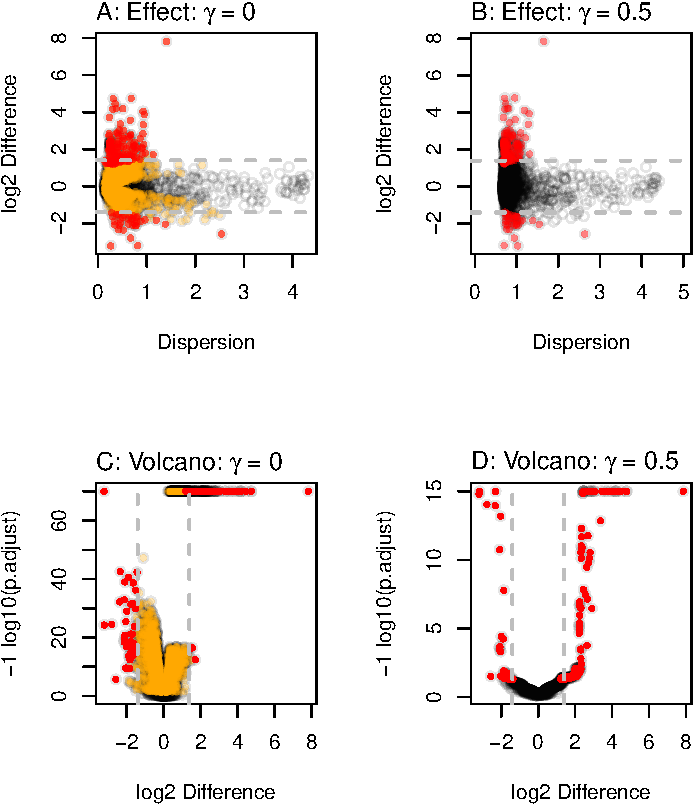
\includegraphics[keepaspectratio]{go3_files/figure-latex/plot1-1.pdf}}
\caption{Volcano and effect plots for unscaled and scaled transcriptome
analysis. ALDEx2 was used to conduct a differential expression (DE)
analysis on the yeast transcriptome dataset. The results were plotted to
show the relationship between difference and dispersion using effect
plots or difference and the q-values using volcano plots. Panels A,C are
for the naive analyses, and Panels B,D are for the default analyses that
include scale uncertainty. Each point represents the values for one
transcript, with the color indicating if that transcript was significant
in the both analyses (red) or in the naive analysis only (orange).
Points in grey are not statistically signficantly different under any
condition. The horizontal dashed lines represent a \(\log_2\)difference
of \(\pm 1.4\).}
\end{figure}

The Volcano plots in Figure 1 A and B show that adding scale uncertainty
increases the minimum q-value and increases the concordance between the
q-value and the difference between groups (compare panels A and B). The
effect plots (44) in Figure 1C shows that the majority of significant
transcripts (red, orange) have negligible differences between groups and
very low dispersion. We suggest that this low dispersion is driven by
the experimental design which is actually a technical wet lab
replication rather than a true biological replication design (41). Scale
uncertainty can be incorporated using the \texttt{gamma} parameter that
controls the amount of noise added to the CLR mean assumption when we
call either \texttt{aldex()}, or \texttt{aldex.clr()}. Figure 1 B,D
shows that setting \(\gamma=0.5\) results in 205 which is far fewer
significant transcripts than in the naive analysis and we observe that
the minimum dispersion increases from 0.12 (\(\gamma = 0\) ) to 0.67
(\(\gamma=0.5\)).

\begin{figure}
\centering
\pandocbounded{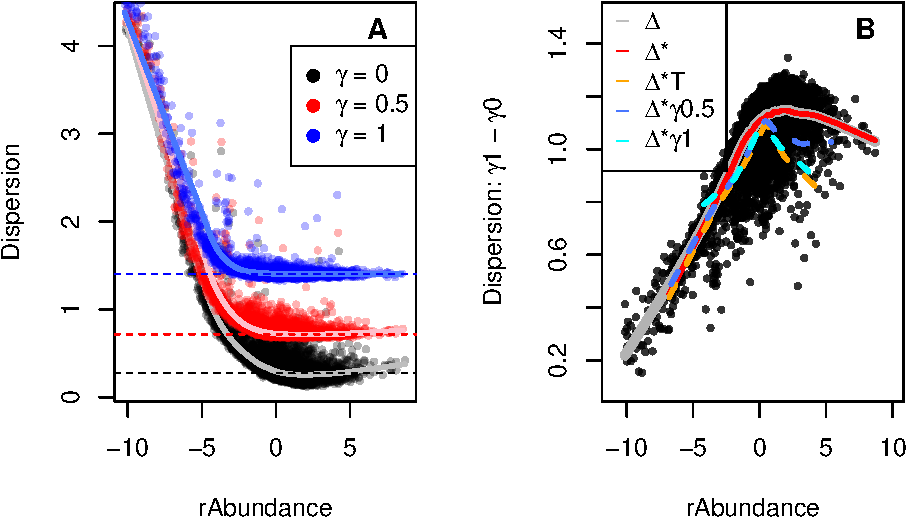
\includegraphics[keepaspectratio]{go3_files/figure-latex/disp-1.pdf}}
\caption{Adding scale uncertainty changes the dispersion distribution.
Panel A shows a plot of the expected value for relative abundance vs the
expected value for the pooled dispersion as output by
\texttt{aldex.effect}. The dashed horizontal lines show the median value
for the features with a rAbundance between -0.5 and 0.5, and the light
colored lines are lowess lines of fit through the center of mass of the
data. Panel B plots the dispersion difference between \(\gamma = 1\) and
\(\gamma = 0\); note the non-linear relationship that highlights the
rotation that is evident in Panel A. The colored lines indicate the
lowess line of fit through the centre of mass of the plot for the
various populations of points. The grey line is the total population and
shows the difference \(\Delta\), the red line is the population of
significant transcripts (*) with \(\gamma = 0\), the orange line is the
population of significant transcripts with a difference threshold (T) of
about \(\pm 2^{1.4}\)-fold change, the blue line is the population of
significant transcripts with \(\gamma = 0.5\), and the cyan line is the
significant population with \(\gamma = 1\). \(\Delta\): Difference, *:
significant, T: thresholded.}
\end{figure}

It is common practice to use a dual-cutoff by choosing transcripts based
on a thresholds for both q-values and fold-changes (10, 12). Note that
there is considerable variation in recommended cutoff values(10). Here,
applying a dual-cutoff using a heuristic of at least a \(2^{1.4}\) fold
change reduces the number of significant outputs to 193 for DESeq2 and
to 186 for ALDEx2. This cutoff was chosen for convenience and is in-line
with the recommendations of (10). the fold change limits are shown by
the dashed grey lines in Figure 1. The \(2^{1.4}\) fold change cutoff
identifies a similar number of transcripts as does ALDEx2 using
\(\gamma = 0.5\) which identifies 205. Supplementary Figure 2 shows how
to use the \texttt{aldex.senAnalysis()} function to identify those
transcripts that are very sensitive to scale uncertainty. In this
supplementary figure we see that even adding a very small amount of
scale \(\gamma = 0.1\) reduces the number of significant transcripts by
more than half. This allows us to those low-dispertion transcripts that
were significant only because of an absence of scale uncertainty. In
practice, we suggest that a \texttt{gamma} parameter between 0.5 and 1
is realistic for most experimental designs (16).

The effect on dispersion with increasing amounts of scale uncertainty
are shown in Figure 2A, where we can see that the dispersion increases
as uncertainty is added. Note that the dispersion in the unscaled
analysis in Figure 2A reaches a minimum near the mid-point of the
distribution, and also does so when the analysis is conducted with
DESeq2 (Supplementary Figure 3). This shows more clearly that dispersion
of many transcripts is almost negligible in the absence of scale
uncertainty. This plot makes the counter-intuitive suggestion that the
variance in expression of the majority of genes with moderate expression
is more predictable than highly-expressed genes or of housekeeping genes
(45). This is at odds with the known biology of cells where single cell
counting of highly-expressed transcripts shows that they have little
intrinsic variation (20, 46).

Adding scale uncertainty by setting \(\gamma=0.5\) , or
\(\gamma = 1.0\), increases the minimum dispersion as shown in Figure 2A
by the red and blue data points, and by the colored lines of fit through
the centre of mass of the data. Less obvious is that the additional
dispersion is not applied equally to all points. Figure 2B shows a plot
of the difference between the \(\gamma= 0\) and \(\gamma= 1\) data and
here we can see that scale uncertainty is preferentially increasing the
dispersion of the mid-expressed transcripts that formerly had negligible
dispersion; examine the grey line of best fit (overlaid by the red line)
for the trend. Panel B also shows the trend of the expression-dispersion
relationship for transcripts that are classed as statistically
significant. The red line shows the trendline with no added scale
uncertainty, and this trendline exactly overlays with the grey trendline
for the bulk of transcripts. The orange trendline indicates those
transcripts that are both statistically significant and that have a
thresholded expression level of \(\pm 1.4\), and the dark blue and cyan
lines show the statistically significant trendline for \(\gamma=0.5\) ,
or \(1.0\).

Thus, taking Figures 1 and 2 together adding scale uncertainty has the
desirable effect of changing the distribution of transcripts identified
as significantly different between groups. Those parts that were
statistically significantly different \emph{only because of low
dispersion} are preferentially excluded from statistical significance
while those parts that were significantly different because of a high
difference between groups remain.

\subsection{Housekeeping genes and functions to guide scale model
choices.}\label{housekeeping-genes-and-functions-to-guide-scale-model-choices.}

Dos Santos et al. (47) used a vaginal metatranscriptome dataset to
compare the gene expression in bacteria collected from healthy (H) and
bacterial vaginosis (BV) affected women. In this environment, both the
relative abundance of species between groups and the gene expression
level within a species is different (48). Additionally, prior research
suggests that the total number of bacteria is about 10 times more in the
BV than in the H condition (23). Thus, these are extremely challenging
datasets in which to determine differential abundance as there are both
compositional and scale changes between conditions. The usual method to
analyze vaginal metratranscriptome data is to do so on an
organism-by-organism basis (48--50) because the scale confounding of the
environment is less pronounced. One attempt at system-wide analysis
returned several housekeeping functions as differentially expressed
between groups (49); a result likely due to a disconnect between the
assumptions of the normalization used and the actual scale of the
environment (15).

In this example, we show how to specify and interpret an informed scale
model that can explicitly account for some of these modeling
difficulties (16) even in a difficult dataset. An informed scale model
can control for both the mean difference of scale between groups (e.g.,
directly incorporate information on the differences in total number of
bacteria between the BV and H conditions) as well as the uncertainty of
that difference. To specify a user-defined scale model, we can pass a
matrix of scale values instead of an estimate of just the scale
uncertainty to \texttt{aldex.clr()}. This matrix should have the same
number of rows as the of Monte-Carlo Dirichlet samples, and the same
number of columns as the number of samples. While this matrix can be
computed from scratch by the analyst, there is an
\texttt{aldex.makeScaleModel()} function that can be used to simplify
this step in most cases. This encodes the scale model as
\(\Lambda \sim N(log_2 \mu_n, \gamma^{2})\), where \(\mu_n\) represents
the scale value for each sample or group and gamma is the uncertainty as
before. The scale estimate can be a measured value (cell count, nucleic
acid input, etc) or an estimate. Nixon et al. (16) showed that only the
ratio of the means are important when providing values for \(\mu_n\);
i.e., the ratio between the \(\log_2 \mu_i\) and \(\log_2 \mu_j\)
values. See the supplement to Nixon et al. (16) for more information.

Figure 3A shows an effect plot of the data where reads are grouped by
homologous sequence regardless of the organism of origin. Each point
represents one of 3728 KEGG functions (51). There are many more
functions represented in the BV group (bottom) than in the healthy group
(top). This is because the \textit{Lactobacilli} that dominate a healthy
vaginal microbiome have reduced genome content relative to the anaerobic
organisms that dominate in BV, because there is a greater diversity of
organisms in BV than in H samples, and because the BV condition has at
least an order of magnitude more bacteria than does the H condition.

There are 101 functions with low dispersion that appear to be shared by
both groups (boxed area in Figure 3A, and colored in cyan). Inspection
shows that these largely correspond to core metabolic functions such as
transcription, translation, ribosomal proteins, glycolysis, replication,
chaperones, etc (Supplementary file housekeeping.txt). The transcripts
of many of these are commonly used as invariant reference sequences in
wet lab experiments (45) and so are not be expected to contribute to
differences in ecosystem behaviour. The average location of these should
be centred on 0 difference to represent an internal reference set.
However, without an informed scale model, the mean of these housekeeping
functions is approximately located at +2.3.

\begin{figure}
\centering
\pandocbounded{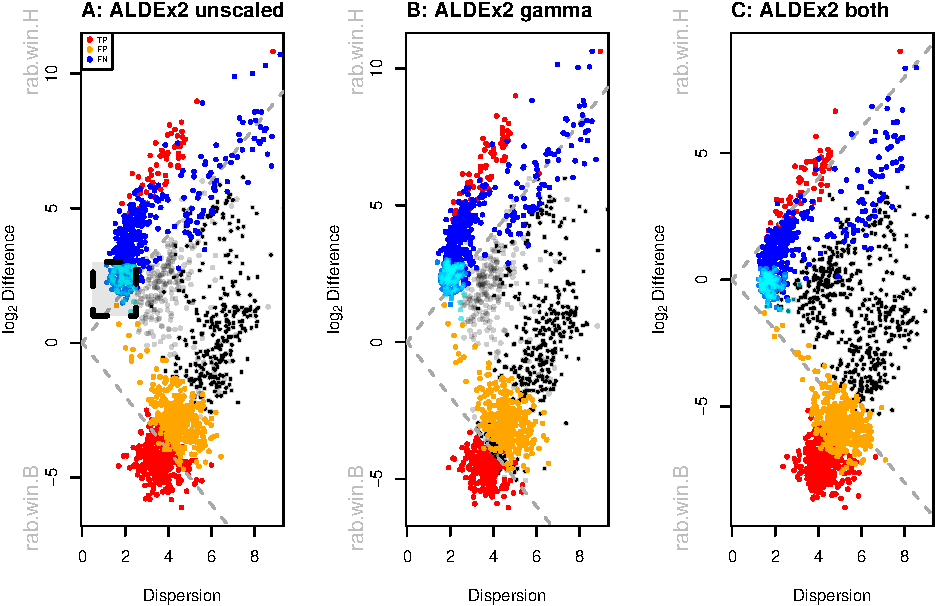
\includegraphics[keepaspectratio]{go3_files/figure-latex/meta-1.pdf}}
\caption{Analysis of vaginal transcriptome data aggregated at the Kegg
Orthology (KO) functional level. Panel A shows an effect plot for the
default analysis where the functions that are elevated in the healthy
individuals have positive values and functions that are elevated in BV
have negative values. Highlighed in the box are KOs that are almost
exlusively housekeeping functions; these and are colored cyan. These
housekeeping functions should be located on the midline of no
difference. Panel B shows the same data scaled with \(\gamma = 0.5\),
which increase the minimum dispersion as before. Panel C shows the same
data scaled with \(\gamma = 0.5\) and a 0.14 fold difference in
dispersion applied to the BV samples relative to the H samples. In these
plots statistically significant (q-value \textless{} 0.01) functions in
the informed model are in red, false positive functions are in blue,
non-significant functions in black and false negative functions are in
orange.}
\end{figure}

Applying the default scale model of \(\gamma=0.5\) increases the
dispersion slightly but does not move the housekeeping functions toward
the midline. This is as expected; the mean of the default scale model is
based on the CLR normalization so no shift in location would be expected
over the original ALDEx2 model. Nevertheless, about 30\% of the
housekeeping functions are no longer statistically significantly
different. Note that this change is simple to conduct, has no additional
computational complexity and requires only a slight modification for the
analyst.

We desire a scale model that approximately centres the housekeeping
functions. Our starting point for this is to identify the naive scale
estimate from the data, and this can be done by calculating the mean
scale value for each group with a negligible scale value; i.e.,
\(\gamma=1e-3\). The scale estimate for samples can be accessed in the
\texttt{@scaleSamps} slot from the \texttt{aldex.clr} output. In this
datset the naive scale estimate for the healthy group is 17.41 and for
the BV group is 14.59 for a difference of 2.82. This is interpreted as
the scale of the H group of samples being 7.06 greater than the BV
group. This precise but incorrect estimate places the location of the
housekeeping genes off the midline of no difference.

We anticipate that housekeeping functions should be nearly invariant and
so an appropriate scale in this dataset is likely closer to 0 than the
naive estimate. One way to choose an appropriate value for \(\mu_n\) is
to us the \texttt{aldex.clr} function on only the presumed invariant
functions setting \(\gamma > 0\), and then accessing the
\texttt{@scaleSamps} slot as before. Doing so suggests that the
difference in scale should be about 14\%. A second approach would be to
identify the functions used as the denominator with the
\texttt{denom="lvha"} option (15) for the \texttt{aldex.clr} function,
and then to use these values as before. This approach suggests a 5\%
difference in scale, and is potentially less subject to user
interpretation.

For the purposes of this example, if we assume a 14\% difference in
scale, we can set \(\mu_i = 1\) and \(\mu_j = 1.14\) using the
\texttt{makeScaleMatrix} function. This function uses a logNormal
distribution to build a scale matrix given a user-specified mean
difference between groups and uncertainty level. Applying a per-group
relative differential scale of 0.14 moves the housekeeping functions to
the midline of no difference (Figure 3C, 14\% mean difference = -0.24,
5\% difference = -0.34), and applying a gamma of 0.5 provides the same
dispersion as in panel B of Figure 3. Note that now a significant number
of functions are differentially up in BV that were formerly classed as
not different without the full scale model (orange), or when only a
default scale was applied. Inspection of the functions shows that these
are largely missing from the \emph{Lactobacillus} species and so should
actually be captured as differentially abundant in the BV group. The
supplement shows that the using either the 5\% or the 14\% scale
difference give imperceptibly different results suggesting that an
informed scale model does not have to precisely estimate the scale
difference to be useful. Nixon et al, (16) found that multiple
reasonable estimates for the \(\mu_n\) part of the informed scale model
were similarly useful in microbiome data.

Thus, applying an informed scale allows us to distinguish between both
false positives (housekeeping functions in cyan, and others in blue) and
false negatives (orange functions) even in a very difficult to analyze
dataset. The remarkable improvements in biological interpretation
afforded by an informed scale model, and the transferrability of it
between sample cohorts of the same condition is outlined elsewhere (47).
We suggest that the default scale model is sufficient when the data are
approximately centred. However, an informed model is more appropriate
with datasets are not well centred or when the investigator has prior
information about the underlying biology.

\section{Discussion}\label{discussion}

Biological systems are both predictably variable and stochastic (46) and
systems biology experiments show that there are transcripts with
approximately constant concentrations in the cell and those with large
variability under different growth conditions (20). Current measurement
methods that rely on high throughput sequencing fail to capture all of
the variation, particularly variation due to scale (3, 16). In the
absence of external information (4, 19, 52) sequencing depth
normalisation methods cannot recapture the scale information (19), and
can only normalize for the technical variation due to sequencing depth.
Here we demonstrated that even approximate estimates of scale and the
uncertainty of measuring it can aid in the interpretation of
RNA-sequencing experiments.

Nixon et al. (3) introduced the idea of explicitly modelling the scale
of a HTS dataset, and showed how to incorporate these models in the
analysis of microbiome and other datasets (16). They demonstrated that
many tools commonly used to analyze HTS datasets had substantial Type 1
and Type 2 error rates, in line with recent findings by others (9). A
version of ALDEx2 with the ability to include scale uncertainty was
shown to be able to correct for the high Type 1 error rate for that
tool, albeit with some loss of sensitivity. Finally, they showed that
incorporating an informed scale model incorporating both location and
scale uncertainty estimates could both control for Type 1 and Type 2
error rates (16).

Building and using a scale model, thus has substantial benefits relative
to the dual cutoff approach that is advocated for many gene expression
experiments (10, 12). In particular, the dual cutoff approach has long
been known to not control for Type 1 errors (13, 14), and the frequent
lack of concordance between tools when benchmarked on transcriptomes(7,
9, 10, 26, 53) and microbiomes (6, 8, 28, 37, 54, 55) suggests poor
control of Type 2 errors as well (7, 9). Thus, incorporating a scale
model during the analysis of HTS data promises the best of both worlds.
A default scale model can control for Type 1 errors with minimal prior
knowledge of the environment and this can be done with essentially no
additional computational overhead. Furthermore, this work and previous
(16) show that even minimal information about the underlying environment
can be used to build a relatively robust scale model that controls for
both Type 1 and 2 error rates.

In the analysis of HTS data it is often observed that larger datasets
converge on the majority of parts being significantly different (3, 9,
10). Li et al. (9) conducted a permutation-based benchmarking study and
found that widely used tools performed worse than simple Wilcoxon
rank-sum tests in controlling the FDR when sample sizes became large.
They suggested that the presence of outliers were one of the factors
driving this observation. Brooks et al. (56) suggested that
inappropriate choice of benchmarking methods are also a major
contributing factor and that objective standards of truth are important.
From the perspective of our work the disagreement between tools can be
explained by the observation that different analytic approaches produce
different parameter estimates. Thus, more data produces worse estimates
because the additional data simply increases the precision of a flawed
estimate (3, 57).

Scale simulation is now build into ALDEx2 (16) and this work suggest
that there are two main root causes to common HTS data pathologies. The
first contributing factor is the observed very low dispersion estimate
for many features that is a by-product of experimental design,
sequencing and normalization. In the Schurch et al. (10) dataset, the
data were from single colonies derived from a single culture. Thus, it
is more accurate to describe the 96 samples as wet-lab technical
replicates rather than independent samples. This type of replication
approach is standard in the molecular literature, and would be expected
to result in the very low dispersion that is observed. Applying the
default scale model with \(\gamma=0.5\) a large number of transcripts
have their dispersion increased (Figure 1D), with the effect being
largest for those with the lowest initial dispersion (Figure 2). Adding
scale uncertainty results in modest number of transcripts, 205, being
called significantly different as shown in the volcano plot in Figure 1B
(red points). In addition, there is now a strong concordance between the
difference and p-values. In hindsight, what is not obvious is why the
unscaled volcano plot shows such poor correspondence. We suggest that
this can be explained by random fluctuations in the many variance
estimates with very low values, and this is supported by the plots shown
in Figure 2.

The second contributing factor is unacknowledged asymmetry in many
datasets (15); i.e., different gene content or a directional change in
the majority of features. In the case of asymmetry, the use of a
user-specified scale model can be very useful for otherwise
difficult-to-analyze datasets such as meta-transcriptomes and in-vitro
selection datasets where the majority of features can change. We showed
one such example for the metatranscriptome dataset in Figure 3. Here the
dataset was highly asymmetrical. Incorporating differential scale on a
per-group basis moves the mass of the housekeeping functions towards the
midline of no difference and so affects both Type I and Type II error
rates. We showed two ways of estimating the scale difference between
groups and found that any reasonable estimate is an improvement over the
default scale model. This is in line with the observations by Nixon et
al (16) in a 16S rRNA gene sequencing dataset. It is also of note that
in the case of true biological replicates (different individuals) that
adding a modest amount of scale \(\gamma=0.5\) had little effect on the
the difference between groups and on the dispersion. Thus, in this
dataset the scale mis-specification was affecting mainly the location of
the difference between groups. While we acknowledge that some prior
information on which housekeeping transcripts should not be classed as
differentially abundant is needed, we suggest that this information is
widely available and is already used when performing the gold-standard
quantitative PCR test of differential abundance (58, 59).

Beyond concerns of fidelity and rigor, scale models also enhance the
reproducibility and transparency of HTS analyses. The addition of scale
uncertainty essentially tests the model over a range of normalizations
(3) and so can replace the consensus approach that has been proposed by
some groups (8, 60) with no additional computational overhead. Thus, an
advantage of incorporating scale is that analyses can be made much more
robust such that actual or potential differences in scale can be tested
and accounted for explicitly. While it is beyond the scope of the
present article, we note that there are many ways of building scale
models that enhance the interpretability of the parameters and
assumptions and a detailed description of these points is describe
elsewhere (3).

In summary, we supply a toolkit that makes incorporating scale
uncertainty and location information simple to incorporate for
transcriptomes or indeed any type of HTS dataset. While the underlying
scale of the system is generally inaccessible, the effect of scale on
the analysis outcomes can be modelled and can help explain some of the
underlying biology, and help to expose known issues with the analysis of
HTS data. Adding scale information to the analysis allows for more
robust inference because the features that are sensitive to scale can be
identified and their impact on conclusions weighted accordingly.
Additionally, the use of informed scale models permits difficult to
analyze datasets to be examined in a robust and principled manner even
when the majority of features are asymmetrically distributed or
expressed (or both) in the groups (47). Thus, using and reporting scale
uncertainty should become a standard practice in the analysis of HTS
datasets.

\singlespacing

\section*{References}\label{references}
\addcontentsline{toc}{section}{References}

\phantomsection\label{refs}
\begin{CSLReferences}{1}{1}
\bibitem[\citeproctext]{ref-lovell:2011}
1. Lovell,D., Müller,W., Taylor,J., Zwart,A. and Helliwell,C. (2011)
Proportions, percentages, ppm: Do the molecular biosciences treat
compositional data right? In Pawlowsky-Glahn,V., Buccianti,A. (eds),
\emph{Compositional Data Analysis: Theory and Applications}. John Wiley;
Sons New York, NY, London, pp. 193--207.

\bibitem[\citeproctext]{ref-Quinn:2019aa}
2. Quinn,T.P., Erb,I., Gloor,G., Notredame,C., Richardson,M.F. and
Crowley,T.M. (2019) \href{https://doi.org/10.1093/gigascience/giz107}{A
field guide for the compositional analysis of any-omics data}.
\emph{Gigascience}, \textbf{8}.

\bibitem[\citeproctext]{ref-nixon2023scale}
3. Nixon,M.P., Letourneau,J., David,L.A., Lazar,N.A., Mukherjee,S. and
Silverman,J.D. (2023) \href{https://arxiv.org/abs/2201.03616}{Scale
reliant inference}. \emph{https://arxiv.org/abs/2201.03616}.

\bibitem[\citeproctext]{ref-Vandeputte:2017aa}
4. Vandeputte,D., Kathagen,G., D'hoe,K., Vieira-Silva,S.,
Valles-Colomer,M., Sabino,J., Wang,J., Tito,R.Y., De Commer,L.,
Darzi,Y., \emph{et al.} (2017)
\href{https://doi.org/10.1038/nature24460}{Quantitative microbiome
profiling links gut community variation to microbial load}.
\emph{Nature}, \textbf{551}, 507--511.

\bibitem[\citeproctext]{ref-Props:2017aa}
5. Props,R., Kerckhof,F.-M., Rubbens,P., De Vrieze,J., Hernandez
Sanabria,E., Waegeman,W., Monsieurs,P., Hammes,F. and Boon,N. (2017)
\href{https://doi.org/10.1038/ismej.2016.117}{Absolute quantification of
microbial taxon abundances}. \emph{ISME J}, \textbf{11}, 584--587.

\bibitem[\citeproctext]{ref-Thorsen:2016aa}
6. Thorsen,J., Brejnrod,A., Mortensen,M., Rasmussen,M.A., Stokholm,J.,
Al-Soud,W.A., Sørensen,S., Bisgaard,H. and Waage,J. (2016)
\href{https://doi.org/10.1186/s40168-016-0208-8}{Large-scale
benchmarking reveals false discoveries and count transformation
sensitivity in 16{S} r{RNA} gene amplicon data analysis methods used in
microbiome studies}. \emph{Microbiome}, \textbf{4}, 62.

\bibitem[\citeproctext]{ref-Quinn:2018aa}
7. Quinn,T.P., Crowley,T.M. and Richardson,M.F. (2018)
\href{https://doi.org/10.1186/s12859-018-2261-8}{Benchmarking
differential expression analysis tools for RNA-seq: Normalization-based
vs. Log-ratio transformation-based methods}. \emph{BMC Bioinformatics},
\textbf{19}, 274.

\bibitem[\citeproctext]{ref-Nearing:2022aa}
8. Nearing,J.T., Douglas,G.M., Hayes,M.G., MacDonald,J., Desai,D.K.,
Allward,N., Jones,C.M.A., Wright,R.J., Dhanani,A.S., Comeau,A.M.,
\emph{et al.} (2022)
\href{https://doi.org/10.1038/s41467-022-28034-z}{Microbiome
differential abundance methods produce different results across 38
datasets}. \emph{Nat Commun}, \textbf{13}, 342.

\bibitem[\citeproctext]{ref-Li:2022aa}
9. Li,Y., Ge,X., Peng,F., Li,W. and Li,J.J. (2022)
\href{https://doi.org/10.1186/s13059-022-02648-4}{Exaggerated false
positives by popular differential expression methods when analyzing
human population samples}. \emph{Genome Biol}, \textbf{23}, 79.

\bibitem[\citeproctext]{ref-Schurch:2016aa}
10. Schurch,N.J., Schofield,P., Gierliński,M., Cole,C., Sherstnev,A.,
Singh,V., Wrobel,N., Gharbi,K., Simpson,G.G., Owen-Hughes,T., \emph{et
al.} (2016) \href{https://doi.org/10.1261/rna.053959.115}{How many
biological replicates are needed in an RNA-seq experiment and which
differential expression tool should you use?} \emph{RNA}, \textbf{22},
839--51.

\bibitem[\citeproctext]{ref-storey2003positive}
11. Storey,J.D. (2003) The positive false discovery rate: A bayesian
interpretation and the q-value. \emph{The annals of statistics},
\textbf{31}, 2013--2035.

\bibitem[\citeproctext]{ref-Cui:2003aa}
12. Cui,X. and Churchill,G.A. (2003)
\href{https://www.ncbi.nlm.nih.gov/pubmed/12702200}{Statistical tests
for differential expression in cDNA microarray experiments}.
\emph{Genome Biol}, \textbf{4}, 210.1--210.10.

\bibitem[\citeproctext]{ref-Zhang:2009aa}
13. Zhang,S. and Cao,J. (2009)
\href{https://doi.org/10.1186/1471-2105-10-402}{A close examination of
double filtering with fold change and t test in microarray analysis}.
\emph{BMC Bioinformatics}, \textbf{10}, 402.

\bibitem[\citeproctext]{ref-Ebrahimpoor:2021aa}
14. Ebrahimpoor,M. and Goeman,J.J. (2021)
\href{https://doi.org/10.1093/bib/bbab053}{Inflated false discovery rate
due to volcano plots: Problem and solutions}. \emph{Brief Bioinform},
\textbf{22}.

\bibitem[\citeproctext]{ref-Wu2021}
15. Wu,J.R., Macklaim,J.M., Genge,B.L. and Gloor,G.B. (2021)
\href{https://doi.org/10.1007/978-3-030-71175-7_17}{Finding the centre:
Compositional asymmetry in high-throughput sequencing datasets}. In
Filzmoser,P., Hron,K., Martìn-Fernàndez,J.A., Palarea-Albaladejo,J.
(eds), \emph{Advances in compositional data analysis: Festschrift in
honour of vera pawlowsky-glahn}. Springer International Publishing,
Cham, pp. 329--346.

\bibitem[\citeproctext]{ref-Nixon2024B}
16. Nixon,M.P., Gloor,G.B. and Silverman,J.D. (2024) Beyond
normalization: Incorporating scale uncertainty in microbiome and gene
expression analysis. \emph{bioRxiv},
\href{https://doi.org/10.1101/2024.04.01.587602}{10.1101/2024.04.01.587602}.

\bibitem[\citeproctext]{ref-Lovell:2015}
17. Lovell,D., Pawlowsky-Glahn,V., Egozcue,J.J., Marguerat,S. and
Bähler,J. (2015)
\href{https://doi.org/10.1371/journal.pcbi.1004075}{Proportionality: A
valid alternative to correlation for relative data}. \emph{PLoS Comput
Biol}, \textbf{11}, e1004075.

\bibitem[\citeproctext]{ref-Nie:2012aa}
18. Nie,Z., Hu,G., Wei,G., Cui,K., Yamane,A., Resch,W., Wang,R.,
Green,D.R., Tessarollo,L., Casellas,R., \emph{et al.} (2012)
\href{https://doi.org/10.1016/j.cell.2012.08.033}{C-{M}yc is a universal
amplifier of expressed genes in lymphocytes and embryonic stem cells}.
\emph{Cell}, \textbf{151}, 68--79.

\bibitem[\citeproctext]{ref-Loven:2012aa}
19. Lovén,J., Orlando,D.A., Sigova,A.A., Lin,C.Y., Rahl,P.B.,
Burge,C.B., Levens,D.L., Lee,T.I. and Young,R.A. (2012)
\href{https://doi.org/10.1016/j.cell.2012.10.012}{Revisiting global gene
expression analysis}. \emph{Cell}, \textbf{151}, 476--82.

\bibitem[\citeproctext]{ref-Scott:2010}
20. Scott,M., Gunderson,C.W., Mateescu,E.M., Zhang,Z. and Hwa,T. (2010)
\href{https://doi.org/10.1126/science.1192588}{Interdependence of cell
growth and gene expression: Origins and consequences}. \emph{Science},
\textbf{330}, 1099--102.

\bibitem[\citeproctext]{ref-Yoshikawa:2011aa}
21. Yoshikawa,K., Tanaka,T., Ida,Y., Furusawa,C., Hirasawa,T. and
Shimizu,H. (2011) \href{https://doi.org/10.1002/yea.1843}{Comprehensive
phenotypic analysis of single-gene deletion and overexpression strains
of saccharomyces cerevisiae}. \emph{Yeast}, \textbf{28}, 349--61.

\bibitem[\citeproctext]{ref-Lin:2018aa}
22. Lin,J. and Amir,A. (2018)
\href{https://doi.org/10.1038/s41467-018-06714-z}{Homeostasis of protein
and mRNA concentrations in growing cells}. \emph{Nat Commun},
\textbf{9}, 4496.

\bibitem[\citeproctext]{ref-Zozaya:2010}
23. Zozaya-Hinchliffe,M., Lillis,R., Martin,D.H. and Ferris,M.J. (2010)
\href{https://doi.org/10.1128/JCM.00851-09}{Quantitative PCR assessments
of bacterial species in women with and without bacterial vaginosis}.
\emph{J Clin Microbiol}, \textbf{48}, 1812--9.

\bibitem[\citeproctext]{ref-Ravel:2010}
24. Ravel,J., Gajer,P., Abdo,Z., Schneider,G.M., Koenig,S.S.K.,
McCulle,S.L., Karlebach,S., Gorle,R., Russell,J., Tacket,C.O., \emph{et
al.} (2011) Vaginal microbiome of reproductive-age women. \emph{Proc
Natl Acad Sci U S A},
\href{https://doi.org/doi/10.1073/pnas.100611107}{doi/10.1073/pnas.100611107}.

\bibitem[\citeproctext]{ref-Hummelen:2010}
25. Hummelen,R., Fernandes,A.D., Macklaim,J.M., Dickson,R.J.,
Changalucha,J., Gloor,G.B. and Reid,G. (2010)
\href{https://doi.org/10.1371/journal.pone.0012078}{Deep sequencing of
the vaginal microbiota of women with {HIV}}. \emph{PLoS One},
\textbf{5}, e12078.

\bibitem[\citeproctext]{ref-Bullard:2010}
26. Bullard,J.H., Purdom,E., Hansen,K.D. and Dudoit,S. (2010)
\href{https://doi.org/10.1186/1471-2105-11-94}{Evaluation of statistical
methods for normalization and differential expression in m{RNA-seq}
experiments}. \emph{BMC Bioinformatics}, \textbf{11}, 94.

\bibitem[\citeproctext]{ref-Dillies:2013}
27. Dillies,M.-A., Rau,A., Aubert,J., Hennequet-Antier,C.,
Jeanmougin,M., Servant,N., Keime,C., Marot,G., Castel,D., Estelle,J.,
\emph{et al.} (2013) \href{https://doi.org/10.1093/bib/bbs046}{A
comprehensive evaluation of normalization methods for {Illumina}
high-throughput {RNA} sequencing data analysis}. \emph{Brief Bioinform},
\textbf{14}, 671--83.

\bibitem[\citeproctext]{ref-Weiss:2017aa}
28. Weiss,S., Xu,Z.Z., Peddada,S., Amir,A., Bittinger,K., Gonzalez,A.,
Lozupone,C., Zaneveld,J.R., Vázquez-Baeza,Y., Birmingham,A., \emph{et
al.} (2017)
\href{https://doi.org/10.1186/s40168-017-0237-y}{Normalization and
microbial differential abundance strategies depend upon data
characteristics}. \emph{Microbiome}, \textbf{5}, 27.

\bibitem[\citeproctext]{ref-Hughes:2005tu}
29. Hughes,J.B. and Hellmann,J.J. (2005)
\href{https://doi.org/10.1016/S0076-6879(05)97017-1}{The application of
rarefaction techniques to molecular inventories of microbial diversity}.
\emph{Methods Enzymol}, \textbf{397}, 292--308.

\bibitem[\citeproctext]{ref-Mortazavi:2008}
30. Mortazavi,A., Williams,B.A., McCue,K., Schaeffer,L. and Wold,B.
(2008) \href{https://doi.org/10.1038/nmeth.1226}{Mapping and quantifying
mammalian transcriptomes by {RNA-seq}}. \emph{Nat Methods}, \textbf{5},
621--8.

\bibitem[\citeproctext]{ref-wagner:tpm}
31. Wagner,G.P., Kin,K. and Lynch,V.J. (2012)
\href{https://doi.org/10.1007/s12064-012-0162-3}{Measurement of mRNA
abundance using RNA-seq data: RPKM measure is inconsistent among
samples}. \emph{Theory Biosci}, \textbf{131}, 281--5.

\bibitem[\citeproctext]{ref-Robinson:2010a}
32. Robinson,M.D. and Oshlack,A. (2010)
\href{https://doi.org/10.1186/gb-2010-11-3-r25}{A scaling normalization
method for differential expression analysis of {RNA-seq} data}.
\emph{Genome Biol}, \textbf{11}, R25.1--R25.9.

\bibitem[\citeproctext]{ref-aitchison1982}
33. Aitchison,J. (1982) The statistical analysis of compositional data.
\emph{Journal of the Royal Statistical Society: Series B
(Methodological)}, \textbf{44}, 139--160.

\bibitem[\citeproctext]{ref-Anders:2010}
34. Anders,S. and Huber,W. (2010)
\href{https://doi.org/10.1186/gb-2010-11-10-r106}{Differential
expression analysis for sequence count data}. \emph{Genome Biol},
\textbf{11}, R106.

\bibitem[\citeproctext]{ref-Aitchison:1986}
35. Aitchison,J. (1986) The statistical analysis of compositional data
Chapman \& Hall, London, England.

\bibitem[\citeproctext]{ref-fernandes:2013}
36. Fernandes,A.D., Macklaim,J.M., Linn,T.G., Reid,G. and Gloor,G.B.
(2013) \href{https://doi.org/10.1371/journal.pone.0067019}{ANOVA-like
differential expression (ALDEx) analysis for mixed population RNA-seq}.
\emph{PLoS One}, \textbf{8}, e67019.

\bibitem[\citeproctext]{ref-Yerke:2024aa}
37. Yerke,A., Fry Brumit,D. and Fodor,A.A. (2024)
\href{https://doi.org/10.1186/s40168-023-01747-z}{Proportion-based
normalizations outperform compositional data transformations in machine
learning applications}. \emph{Microbiome}, \textbf{12}, 45.

\bibitem[\citeproctext]{ref-Love:2014aa}
38. Love,M.I., Huber,W. and Anders,S. (2014)
\href{https://doi.org/10.1186/s13059-014-0550-8}{Moderated estimation of
fold change and dispersion for RNA-seq data with DESeq2}. \emph{Genome
Biol}, \textbf{15}, 550.1--550.21.

\bibitem[\citeproctext]{ref-Paulson:2013aa}
39. Paulson,J.N., Stine,O.C., Bravo,H.C. and Pop,M. (2013)
\href{https://doi.org/10.1038/nmeth.2658}{Differential abundance
analysis for microbial marker-gene surveys}. \emph{Nat Methods},
\textbf{10}, 1200--2.

\bibitem[\citeproctext]{ref-fernandes:2014}
40. Fernandes,A.D., Reid,J.N., Macklaim,J.M., McMurrough,T.A.,
Edgell,D.R. and Gloor,G.B. (2014)
\href{https://doi.org/10.1186/2049-2618-2-15}{Unifying the analysis of
high-throughput sequencing datasets: Characterizing {RNA}-seq, 16{S}
r{RNA} gene sequencing and selective growth experiments by compositional
data analysis}. \emph{Microbiome}, \textbf{2}, 15.1--15.13.

\bibitem[\citeproctext]{ref-Gierlinski:2015aa}
41. Gierliński,M., Cole,C., Schofield,P., Schurch,N.J., Sherstnev,A.,
Singh,V., Wrobel,N., Gharbi,K., Simpson,G., Owen-Hughes,T., \emph{et
al.} (2015)
\href{https://doi.org/10.1093/bioinformatics/btv425}{Statistical models
for RNA-seq data derived from a two-condition 48-replicate experiment}.
\emph{Bioinformatics}, \textbf{31}, 3625--3630.

\bibitem[\citeproctext]{ref-benjamini:1995}
42. Benjamini,Y. and Hochberg,Y. (1995) Controlling the false discovery
rate: A practical and powerful approach to multiple testing.
\emph{Journal of the Royal Statistical Society. Series B
(Methodological)}, \textbf{57}, 289--300.

\bibitem[\citeproctext]{ref-efron2008FDR}
43. Efron,B. (2008) Microarrays, empirical bayes and the two-groups
model. \emph{Statist. Sci.}, \textbf{23}, 1--22.

\bibitem[\citeproctext]{ref-gloor:effect}
44. Gloor,G., Macklaim,J. and Fernandes,A. (2016)
\href{https://doi.org/10.1080/10618600.2015.1131161}{Displaying
variation in large datasets: Plotting a visual summary of effect sizes}.
\emph{Journal of Computational and Graphical Statistics}, \textbf{25},
971--979.

\bibitem[\citeproctext]{ref-Rocha:2020aa}
45. Rocha,D.J.P.G., Castro,T.L.P., Aguiar,E.R.G.R. and Pacheco,L.G.C.
(2020) \href{https://doi.org/10.1007/978-1-4939-9833-3_10}{Gene
expression analysis in bacteria by RT-qPCR}. \emph{Methods Mol Biol},
\textbf{2065}, 119--137.

\bibitem[\citeproctext]{ref-Taniguchi:2010aa}
46. Taniguchi,Y., Choi,P.J., Li,G.-W., Chen,H., Babu,M., Hearn,J.,
Emili,A. and Xie,X.S. (2010)
\href{https://doi.org/10.1126/science.1188308}{Quantifying e. Coli
proteome and transcriptome with single-molecule sensitivity in single
cells}. \emph{Science}, \textbf{329}, 533--8.

\bibitem[\citeproctext]{ref-dosSantos:2024}
47. Dos Dos Santos,S.J., Copeland,C., Macklaim,J.M., Reid,G. and
Gloor,G.B. (2024) Vaginal metatranscriptome meta-analysis reveals
functional BV subgroups and novel colonisation strategies.
\emph{bioRxiv},
\href{https://doi.org/10.1101/2024.04.24.590967}{10.1101/2024.04.24.590967}.

\bibitem[\citeproctext]{ref-macklaim:2013}
48. Macklaim,J.M., Fernandes,A.D., Di Bella,J.M., Hammond,J.-A., Reid,G.
and Gloor,G.B. (2013)
\href{https://doi.org/10.1186/2049-2618-1-12}{Comparative meta-{RNA}-seq
of the vaginal microbiota and differential expression by lactobacillus
iners in health and dysbiosis}. \emph{Microbiome}, \textbf{1}, 12.

\bibitem[\citeproctext]{ref-Denge00262-18}
49. Deng,Z.-L., Gottschick,C., Bhuju,S., Masur,C., Abels,C. and
Wagner-Döbler,I. (2018)
\href{https://doi.org/10.1128/mSphereDirect.00262-18}{Metatranscriptome
analysis of the vaginal microbiota reveals potential mechanisms for
protection against metronidazole in bacterial vaginosis}.
\emph{mSphere}, \textbf{3}.

\bibitem[\citeproctext]{ref-Fettweis:2019aa}
50. Fettweis,J.M., Serrano,M.G., Brooks,J.P., Edwards,D.J., Girerd,P.H.,
Parikh,H.I., Huang,B., Arodz,T.J., Edupuganti,L., Glascock,A.L.,
\emph{et al.} (2019)
\href{https://doi.org/10.1038/s41591-019-0450-2}{The vaginal microbiome
and preterm birth}. \emph{Nat Med}, \textbf{25}, 1012--1021.

\bibitem[\citeproctext]{ref-Okuda:2008}
51. Okuda,S., Yamada,T., Hamajima,M., Itoh,M., Katayama,T., Bork,P.,
Goto,S. and Kanehisa,M. (2008)
\href{https://doi.org/10.1093/nar/gkn282}{KEGG atlas mapping for global
analysis of metabolic pathways}. \emph{Nucleic Acids Res}, \textbf{36},
W423--6.

\bibitem[\citeproctext]{ref-yeast-absolute}
52. Marguerat,S., Schmidt,A., Codlin,S., Chen,W., Aebersold,R. and
Bähler,J. (2012)
\href{https://doi.org/10.1016/j.cell.2012.09.019}{Quantitative analysis
of fission yeast transcriptomes and proteomes in proliferating and
quiescent cells}. \emph{Cell}, \textbf{151}, 671--83.

\bibitem[\citeproctext]{ref-Soneson:2013}
53. Soneson,C. and Delorenzi,M. (2013)
\href{https://doi.org/10.1186/1471-2105-14-91}{A comparison of methods
for differential expression analysis of {RNA-seq} data}. \emph{BMC
Bioinformatics}, \textbf{14}, 91.

\bibitem[\citeproctext]{ref-McMurdie:2014a}
54. McMurdie,P.J. and Holmes,S. (2014)
\href{https://doi.org/10.1371/journal.pcbi.1003531}{Waste not, want not:
Why rarefying microbiome data is inadmissible}. \emph{PLoS Comput Biol},
\textbf{10}, e1003531.

\bibitem[\citeproctext]{ref-hawinkel2017}
55. Hawinkel,S., Mattiello,F., Bijnens,L. and Thas,O. (2018)
\href{http://dx.doi.org/10.1093/bib/bbx104}{A broken promise :
Microbiome differential abundance methods do not control the false
discovery rate}. \emph{BRIEFINGS IN BIOINFORMATICS}.

\bibitem[\citeproctext]{ref-Brooks:2024aa}
56. Brooks,T.G., Lahens,N.F., Mrčela,A. and Grant,G.R. (2024)
\href{https://doi.org/10.1038/s41576-023-00679-6}{Challenges and best
practices in omics benchmarking}. \emph{Nat Rev Genet}, \textbf{25},
326--339.

\bibitem[\citeproctext]{ref-gustafson2015bayesian}
57. Gustafson,P. (2015) Bayesian inference for partially identified
models: Exploring the limits of limited data CRC Press.

\bibitem[\citeproctext]{ref-Thellin:1999aa}
58. Thellin,O., Zorzi,W., Lakaye,B., De Borman,B., Coumans,B.,
Hennen,G., Grisar,T., Igout,A. and Heinen,E. (1999)
\href{https://www.ncbi.nlm.nih.gov/pubmed/10617337}{Housekeeping genes
as internal standards: Use and limits}. \emph{J Biotechnol},
\textbf{75}, 291--5.

\bibitem[\citeproctext]{ref-SEQCux2fMAQC-III-Consortium:2014aa}
59. SEQC/MAQC-III Consortium (2014)
\href{https://doi.org/10.1038/nbt.2957}{A comprehensive assessment of
RNA-seq accuracy, reproducibility and information content by the
sequencing quality control consortium}. \emph{Nat Biotechnol},
\textbf{32}, 903--14.

\bibitem[\citeproctext]{ref-Song:2023aa}
60. Song,H., Ling,W., Zhao,N., Plantinga,A.M., Broedlow,C.A.,
Klatt,N.R., Hensley-McBain,T. and Wu,M.C. (2023)
\href{https://doi.org/10.1186/s12859-023-05147-w}{Accommodating multiple
potential normalizations in microbiome associations studies}. \emph{BMC
Bioinformatics}, \textbf{24}, 22.

\end{CSLReferences}

\end{document}
